\seite{}{Explizite Einschrittverfahren}\anchorpage{1}{neu2}{2 · Explizite Einschrittverfahren und moderne Schrittweitenadaption}\ey{KAPITEL 2}\ptitle{Explizite Einschrittverfahren und moderne Schrittweitenadaption}
Ein warmer Fühler kühlt zunächst rasch ab. Der Tangentenpfeil am Anfang eines langen Schritts zeigt steiler nach unten als am Ende. Wo innerhalb des Schritts sollte man weitere Steigungen messen, und woran erkennt der Rechner, ob sich diese Arbeit gelohnt hat?
\subt{Der Weg durch das Kapitel}
{\tblstart\begin{tabularx}{\linewidth}{@{}Yr@{}}\toprule
\hyperlink{abs2-1}{2.1 · Runge–Kutta-Verfahren konstruieren} & \pagelink{abs2-1}\\[2pt]
\hyperlink{abs2-2}{2.2 · Lokaler Fehler und eingebettete Paare} & \pagelink{abs2-2}\\[2pt]
\hyperlink{abs2-3}{2.3 · Schrittweitensteuerung und dichte Ausgabe} & \pagelink{abs2-3}\\[2pt]
\bottomrule\end{tabularx}\par}
\par\vfill{\centering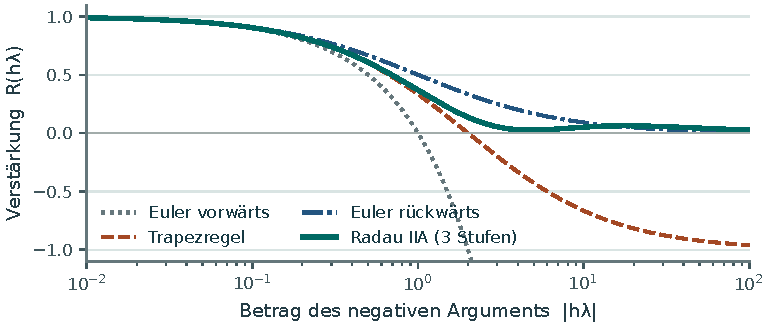
\includegraphics[width=.88\linewidth,height=49mm,keepaspectratio]{stabil.pdf}\par}\capline{Ein Schritt kann die physikalische Dämpfung umkehren.}
\seite{}{Explizite Einschrittverfahren}\anchorpage{2}{abs2-1}{2.1 · Runge–Kutta-Verfahren konstruieren}\ey{ABSCHNITT 2.1}\ptitle{Runge–Kutta-Verfahren konstruieren}
\hypertarget{punkt2-1-1}{}\subt{2.1.1\enspace Zwischenstufen als vorläufige Zustände}
Am beheizten Stab berechnet die erste Stufe die momentane Erwärmung. Mit ihr entwerfen wir einen Zwischenzustand, fragen das physikalische Modell dort erneut und verwenden die Antwort zum Fortschreiben. Die Zwischenzustände sind Versuchswerte. Nur der gewichtete Endwert gelangt in die gespeicherte Bahn.
\hypertarget{punkt2-1-2}{}\subt{2.1.2\enspace Butcher-Tableau und Ordnungsbedingungen}
Ein explizites Tableau speichert \(c_i=\sum_{j<i}a_{ij}\), die Stufen \(k_i=f(t_n+c_ih,y_n+h\sum_{j<i}a_{ij}k_j)\) und die Gewichte \(b_i\). Für konstantes Feld muss \(\sum b_i=1\) gelten. Für \(y'=t\) ist die Steigung linear, ihre exakte Fläche erzwingt \(\sum b_ic_i=1/2\). Ordnung drei verlangt zusätzlich \(b^Tc^2=1/3,\ b^TAc=1/6\), wobei \(c^2\) komponentenweise gilt. Die beiden Bedingungen unterscheiden Zeitkrümmung von einer geschachtelten Rückkopplung.
\hypertarget{punkt2-1-3}{}\subt{2.1.3\enspace Heun, Kutta dritter Ordnung und klassisches RK4}
Heun mittelt Startsteigung und Steigung am Euler-Endpunkt. Kutta-3 verwendet \(c=(0,1/2,1)\), Stufenzeilen \((1/2)\), \((-1,2)\) und Gewichte \((1,4,1)/6\). Bei RK4 folgen auf die Startsteigung zwei Mittelpunktssteigungen und eine Endsteigung. Die Gewichte sind \((1,2,2,1)/6\). Die vier Stufen am realen Heizmodell stehen auf S.\,\pagelink{zeit}. Für \(y'=-y,\ y_0=1,\ h=1\) liefern die drei Verfahren \(1/2,1/3,3/8\). Der Vergleichswert \(e^{-1}\) zeigt, weshalb ein guter erster Schritt noch keine beobachtete Ordnung beweist.
\seite{Rechenbeispiel}{Explizite Einschrittverfahren}\anchorpage{2}{kap4}{Wie baut man aus Steigungen einen Zeitschritt?}\ptitle{Wie baut man aus Steigungen einen Zeitschritt?}


\lernziel{Sie können Euler und Heun selbst ausführen und erklären, wann Genauigkeit, Stabilität oder der Aufwand eines impliziten Schritts die Solverwahl bestimmt.}
Ein Wagen ruht. Während der nächsten Sekunde nimmt seine Beschleunigung gleichmäßig von 0 auf \(2\unitm{m/s^2}\) zu. Was zeigt der Tacho am Ende? Zeichnen Sie die Beschleunigung über der Zeit. Die gesuchte Geschwindigkeitsänderung ist die Fläche unter der Geraden.
\subt{Zwei Rechenregeln, eine unabhängige Kontrolle}
Euler benutzt die Beschleunigung am Anfang. Der Beitrag ist \(1\unitm s\cdot0\unitm{m/s^2}=0\). Für Heun schätzen wir zunächst das Ende mit Euler, werten dort die Beschleunigung aus und mitteln beide Steigungen. Hier hängt die Beschleunigung nur von der Uhr ab. Der Mittelwert ist \((0+2)/2=1\unitm{m/s^2}\), also zeigt der Tacho \(1\unitm{m/s}\).

Die Dreiecksfläche ist unabhängig davon \(\tfrac12\cdot1\cdot2=1\unitm{m/s}\). Heun trifft sie in diesem Sonderfall genau, weil eine Gerade die beiden Messpunkte exakt verbindet. Beim Prüfwagen mit Luftwiderstand hängt die Steigung zusätzlich vom erreichten Tempo ab. Dort müssen wir den Fehler messen.
\notebox{Versuchen Sie einen kleineren Schritt}{Teilen Sie die Sekunde in zwei gleiche Teile. Welche Beschleunigungen sieht Euler an deren Anfängen? Aus \(0{,}5\cdot0+0{,}5\cdot1=0{,}5\unitm{m/s}\) wird sichtbar, was die zweite Auswertung verbessert und welcher Flächenanteil weiterhin fehlt.}
\subt{Wann lohnt die zusätzliche Rechnung?}
Bei einem steilen Abklingen kann ein zu großer Schritt eine abklingende Bewegung sogar wachsen lassen. Die spätere Kontrollrechnung vergleicht deshalb auch den Fehler und die Zahl der nötigen Auswertungen.

\srcs{\textbf{Kernweg}\enspace\see{zeit}{Euler, Heun und RK4}\quad\textbf{Vertiefung}\enspace\see{radau}{Radau-Kollokation}\quad\see{ueb4}{Selbst prüfen}. · \see{pyregler}{In Python ausführen}}

\lektion{Einen Schritt aus Steigungen bauen}{zeit}{Kernweg}{Zeitintegration}
\vorhersage{4}{Ein Wagen steht. Die Zugkraft beginnt bei null und wächst. Was meldet Euler nach seinem ersten Schritt?}{kontrolleA}
Halten Sie die Wärmebilanz des Stabs fest und ändern Sie nur die Schrittregel. Für den Temperaturüberschuss gilt \(\theta(0)=0,\ f(\theta)=(10-\theta/4)/120\). Euler übernimmt \(1/12\unitm{K/s}\) für die ganzen \(60\unitm s\). Das liefert \(5\unitm K\), exakt sind es \(4{,}700124\unitm K\). Die wachsende Wärmeabgabe macht die Anfangssteigung im Laufe des Schritts zu groß.
\subt{Zwischenwerte als Rechenhilfe}
Heuns Verfahren berechnet zuerst den Euler-Prädiktor \(5\unitm K\). Die dortige Steigung ist \((10-5/4)/120=0{,}0729167\unitm{K/s}\). Der Mittelwert aus Anfangs- und Endsteigung liefert \(4{,}6875\unitm K\). Das klassische Runge--Kutta-Verfahren vierter Ordnung (RK4) baut vier Steigungen auf.
{\tblstart\begin{tabularx}{\linewidth}{@{}lYrr@{}}\toprule
\hd{Stufe}&\hd{Auswertung}&\hd{Probezustand [K]}&\hd{Steigung [K/s]}\\\midrule
\(k_1\)& \(f(\theta_0)\)&0&0,08333333\\
\(k_2\)& \(f(\theta_0+hk_1/2)\)&2,500000&0,07812500\\
\(k_3\)& \(f(\theta_0+hk_2/2)\)&2,343750&0,07845052\\
\(k_4\)& \(f(\theta_0+hk_3)\)&4,707031&0,07352702\\\bottomrule
\end{tabularx}\par}
\[
 \theta_1=\theta_0+\frac h6(k_1+2k_2+2k_3+k_4)=4{,}700114\unitm K .
\]
Die zwei Probezustände am halben Schritt erfassen, wie sich die Steigung mit der Temperatur ändert.
\subt{Ein Butcher-Tableau lesen}
Allgemein gilt \(k_i=f(t_n+c_i h,\,y_n+h\sum_j a_{ij}k_j)\) und \(y_{n+1}=y_n+h\sum_i b_i k_i\). Bei RK4 sind \(c=(0,1/2,1/2,1)\), \(b=(1,2,2,1)/6\) und die einzigen von null verschiedenen Einträge \(a_{21}=a_{32}=1/2,\ a_{43}=1\). Die strikte untere Dreiecksform ermöglicht die Auswertung von oben nach unten.
\subt{Warum vier Stufen an der linearen Probe helfen}
Für \(y'=\lambda y\) liefert Einsetzen der vier Stufen den Faktor \(R_4(z)=1+z+z^2/2+z^3/6+z^4/24\), \(z=h\lambda\). Die Exponentialreihe stimmt bis zur vierten Potenz überein. Für dieses Testproblem beginnt der lokale Defekt mit \(z^5y_n/120\). Die allgemeine Ordnung vier für nichtlineare Systeme folgt aus den zusätzlichen RK-Ordnungsbedingungen.
\srcs{\refbk{ode}{Hairer, Nørsett und Wanner, Band I} · Vollständige Zahlen in der eingebetteten Datei \texttt{nachrechnen.py}.}

\lektion{Der Prüfwagen als ODE ohne elementare Lösung}{wagenmodell}{Kernweg}{Zeitintegration}
Ein Prüfwagen startet aus der Ruhe. Sein Antrieb erhöht die Zugkraft jede Sekunde um ein Newton. Gesucht ist die Geschwindigkeit nach einer Sekunde. Darf ein Schalter ansprechen, der \(0{,}48\unitm{m/s}\) verlangt? Ohne Widerstand ergäbe sich \(0{,}5\unitm{m/s}\). Ob uns diese Schätzung für den Schalter genügt, hängt vom Kraftgesetz ab.
\subt{Aus den Kräften zur Gleichung}
Wir modellieren den Wagen als Masse \(m=1\unitm{kg}\). Er fährt waagerecht vorwärts. Ein geschwindigkeitsabhängiger Widerstand wirkt der Bewegung entgegen und beträgt \(c\,v|v|\) mit \(c=1\unitm{kg/m}\). Mit \(\kappa=1\unitm{N/s}\) für die Kraftrampe folgt aus Kraft gleich Masse mal Beschleunigung
\[
 m\dot v=\kappa t-cv|v|,\qquad v(0)=0.
\]
Mit \(s=t/(1\unitm s)\) und \(y=v/(1\unitm{m/s})\) ergibt sich \(y'=s-y|y|\). Für \(s\ge0\) bleibt die Bahn nichtnegativ: Bei \(y=0\) ist die Steigung \(s\), nach dem Start wächst die Geschwindigkeit. Auf unserem Zeitintervall gilt damit \(y'=s-y^2\). Beim Pumpenbeispiel war die Rate allein durch die Uhrzeit bestimmt. Hier bestimmt der erreichte Zustand die nächste Steigung mit.
\subt{Zwei Handrechnungen für die erste halbe Sekunde}
Gehen wir vom Start bis \(s=0{,}5\). Euler übernimmt die Steigung am Start, \(k_1=0-0^2=0\), und erhält wieder \(y=0\). Heun prüft zusätzlich die Steigung am vorhergesagten Ende. Dort liefert \(k_2=0{,}5-0^2=0{,}5\). Aus beiden Steigungen folgt
\[
 y_{\rm Heun}=0+0{,}5\,\frac{0+0{,}5}{2}=0{,}125.
\]
Der Unterschied entsteht schon bei fehlerfrei ausgeführten Rechenoperationen. Während des Schritts wächst die Antriebskraft. Euler verwendet diese Information erst beim nächsten Schritt.
\notebox{Erst schätzen}{Mit Widerstand muss die Geschwindigkeit nach einer Sekunde unter \(0{,}5\unitm{m/s}\) liegen. Reicht diese einseitige Schranke für die Entscheidung bei \(0{,}48\unitm{m/s}\)? Prüfen Sie Ihre Vermutung mit der Tabelle auf der nächsten Seite.}
\srcs{\see{zeit}{Heuns Stufen} · \see{wagenreferenz}{Unabhängige Vergleichsrechnung} · \href{https://pi.math.cornell.edu/~hubbard/diffalg1.pdf}{Hubbard und Lundell, Gleichung (1)}.}

\lektion{Eine unabhängige Antwort für den Prüfwagen}{wagenreferenz}{Kernweg}{Zeitintegration}
Welchen Schalter würde jede der beiden Rechnungen freigeben? Beide bekommen denselben Start und dieselbe Antriebskraft. Die Linearisierung des Widerstands \(y|y|\) bei Ruhe hat Steigung null. Mit \(y'=s\) folgt \(y_\mathrm{lin}=s^2/2\). Die Tabelle stellt diesem Modell die Integration der vollständigen Gleichung gegenüber.
{\tblstart\begin{tabularx}{\linewidth}{@{}r r r r r Y@{}}\toprule
\hd{\(t\) [s]}&\hd{Heun 0,5 s}&\hd{Heun 0,25 s}&\hd{DOP853}&\hd{Referenz}&\hd{Linear}\\\midrule
0,5&0,12500&0,12379&0,12346&0,12346&0,12500\\
1&0,46239&0,45604&0,45554&0,45554&0,50000\\
2&1,16122&1,18695&1,19358&1,19358&2,00000\\\bottomrule\end{tabularx}\par}
Alle Ergebnisse sind Geschwindigkeiten in \(\mathrm{m/s}\). Nach einer Sekunde bleibt das nichtlineare Modell mit \(0{,}45554\unitm{m/s}\) unter der Schwelle. Die Linearisierung würde den Schalter freigeben. Der adaptive DOP853-Lauf verwendet \(\mathrm{rtol}=10^{-11}\), \(\mathrm{atol}=10^{-13}\) und höchstens \(0{,}1\unitm s\) je Schritt.
\subt{Woher die Referenzspalte kommt}
Für \(y=w'/w\) gilt \(y'=w''/w-y^2\). Also genügt es, \(w''=s\,w\) mit \(w(0)=1,\ w'(0)=0\) zu lösen. Dies ist die Airy-Gleichung. Ihre beiden unabhängigen Standardlösungen heißen \(\mathrm{Ai}\) und \(\mathrm{Bi}\). Die Kombination
\[
 W(s)=\mathrm{Bi}'(0)\mathrm{Ai}(s)-\mathrm{Ai}'(0)\mathrm{Bi}(s)
\]
erfüllt \(W'(0)=0,\ W(0)\ne0\). Somit ist \(w=W/W(0)\) und \(y=W'/W\). Für \(s\ge0\) bleibt \(w\) positiv: Solange \(w>0\), ist \(w''=sw\ge0\), also wächst \(w'\) ab null und \(w\) kann keinen ersten Nullpunkt erreichen.
\subt{Warum man die elementare Formel vergeblich sucht}
Für \(y'=s-y^2\) haben Hubbard und Lundell bewiesen, dass sich keine Lösung durch elementare Funktionen darstellen lässt. Ihr Satz schließt sogar weiter gefasste Ausdrücke mit wiederholter Integration und Exponentialbildung aus. Die Spezialfunktionen liefern hier eine exakte Referenz. Die Zeitrechnung kann dasselbe Kraftmodell auch dann weiterverwenden, wenn eine gemessene Kraftrampe die Funktion \(\kappa t\) ersetzt.
\srcs{\texttt{python labor.py wagen} · \href{https://pi.math.cornell.edu/~hubbard/diffalg1.pdf}{Hubbard und Lundell, Einleitung und Korollar 8.1} · \href{https://dlmf.nist.gov/9.2}{NIST DLMF, Airy-Gleichung}.}

\seite{}{Explizite Einschrittverfahren}\anchorpage{2}{abs2-2}{2.2 · Lokaler Fehler und eingebettete Paare}\ey{ABSCHNITT 2.2}\ptitle{Lokaler Fehler und eingebettete Paare}
\hypertarget{punkt2-2-1}{}\subt{2.2.1\enspace Vom lokalen Defekt zum globalen Fehler}
Starten wir auf der exakten Bahn, hinterlässt ein Verfahren der Ordnung \(p\) nach einem Schritt den Defekt \(O(h^{p+1})\). Ein vorhandener Fehler \(e_n\) wird zusätzlich transportiert. Gilt \(\|e_{n+1}\|\le(1+hL)\|e_n\|+Ch^{p+1}\), entsteht durch Aufsummieren einer geometrischen Reihe bei \(e_0=0\) die Schranke \(Ch^p(e^{LT}-1)/L\) für feste Endzeit \(T\) und \(L>0\). Halbieren der Schrittweite prüft diese Beziehung im glatten Problem.
\hypertarget{punkt2-2-2}{}\subt{2.2.2\enspace Zwei Endwerte aus denselben Stufen}
Zwei Gewichtszeilen bilden \(y_{n+1}\) und \(\hat y_{n+1}\) aus denselben ausgewerteten Steigungen. Die Differenz \(h\sum_i(b_i-\hat b_i)k_i\) schätzt im asymptotischen Bereich den führenden lokalen Fehler der niedrigeren Formel. Verschwindet dieser Term ausnahmsweise, kann der Schätzer die Schwierigkeit des folgenden Schritts unterschätzen.
\hypertarget{punkt2-2-3}{}\subt{2.2.3\enspace RK23, RK45 und DOP853 unterscheiden}
Bogacki–Shampine führt eine Lösung dritter Ordnung mit eingebetteter zweiter Ordnung fort. Dormand–Prince 5(4) liefert den verbreiteten RK45. DOP853 ist ein eigenes Verfahren achter Ordnung mit Schätzern fünfter und dritter Ordnung. Jede Formel besitzt eigene Koeffizienten und eine passende dichte Ausgabe. Tauscht man nur den Namen in einem Versuchsbericht aus, lässt sich seine Aufrufzahl kaum interpretieren.
\srcs{\href{https://docs.scipy.org/doc/scipy/reference/generated/scipy.integrate.solve_ivp.html}{SciPy, Löserverfahren und dichte Ausgaben} · \refbk{ode}{Hairer, Nørsett und Wanner}.}
\lektion{Vom lokalen zum globalen Fehler}{ordnung}{Vertiefung}{Zeitintegration}
Ein lokal aus der exakten Lösung gestarteter Euler-Schritt hat bei zweimal stetig differenzierbarer Lösung den Defekt
\[
 y(t+h)-y(t)-hf(t,y(t))=\frac{h^2}{2}y''(\xi),\qquad t<\xi<t+h
\]
für eine skalare Komponente. Ein Verfahren der Ordnung \(p\) hat unter den zugehörigen Glattheitsannahmen einen lokalen Schrittdefekt \(O(h^{p+1})\). Beim Durchmarsch über ein festes Intervall wird der Fehler aus jedem früheren Schritt mittransportiert.
\subt{Satz · Stabile Fehlerfortpflanzung kostet eine Ordnung}
Für eine Einschrittabbildung \(\Phi_h\) gelte \(\|\Phi_h(u)-\Phi_h(v)\|\le(1+Lh)\|u-v\|\) und für jeden exakten Start ein Defekt höchstens \(Kh^{p+1}\). Bei exaktem Anfangswert und \(nh\le T\) folgt
\[
 \|e_n\|\le \frac{K}{L}(e^{LT}-1)h^p\quad (L>0).
\]
\proofpart{Addieren und subtrahieren von \(\Phi_h(y(t_n))\) ergibt \(\|e_{n+1}\|\le(1+Lh)\|e_n\|+Kh^{p+1}\). Iteration ab \(e_0=0\) und Summation der geometrischen Reihe liefern \(Kh^p((1+Lh)^n-1)/L\). Wegen \(1+Lh\le e^{Lh}\) folgt die Schranke. Für \(L=0\) ergibt direktes Summieren \(KTh^p\).}
\subt{Ordnung beobachten}
Halbiert man bei festem Endzeitpunkt \(h\), so ergibt \(p_\mathrm{obs}=\log_2(E_h/E_{h/2})\) einen Schätzwert für die Ordnung. Dazu müssen dieselbe Messgröße, dieselbe Referenz und derselbe Endzeitpunkt verwendet werden. Für Euler, Heun und RK4 erwartet man an einem glatten ODE-Problem asymptotisch die Werte 1, 2 und 4.

In einer Stoßrechnung gilt die glatte Fehlerentwicklung nur innerhalb einer Flugphase. Wird der Stoß verspätet behandelt, beginnt die nächste Phase bereits mit einem anderen Anfangswert. Eine kleine lokale Fehlerschätzung ersetzt deshalb keinen Vergleich der Stoßzeiten.
\task{3}{Für \(\dot y=-y,\ y(0)=1\) führt Euler einen Schritt \(h=1\) oder zwei Schritte \(h=1/2\) aus. Berechnen Sie beide Endwerte und Fehler. Wie lautet die exakte Euler-Folge bis \(t=1\) für \(n\) Schritte?}

\lektion{Was eine adaptive Toleranz steuert}{adaptiv}{Kernweg}{Zeitintegration}
Ein eingebettetes Runge--Kutta-Paar nutzt dieselben Stufen mit zwei verschiedenen Endgewichten. Beim Bogacki--Shampine-Paar RK23 hat die fortgeschriebene Lösung Ordnung 3, die Vergleichslösung Ordnung 2. Für ihre Differenz gilt bei glatter Lösung typischerweise \(\delta\sim K h^3\).
\[
 \begin{array}{c|cccc}
 0&&&&\\
 1/2&1/2&&&\\
 3/4&0&3/4&&\\
 1&2/9&1/3&4/9&\\ \hline
 b^{(3)}&2/9&1/3&4/9&0\\
 b^{(2)}&7/24&1/4&1/3&1/8
 \end{array}
\]
Die letzte Stufe liegt am vorgeschlagenen Endzustand. Nach Annahme des Schritts kann die dortige Steigung beim nächsten Schritt wiederverwendet werden, solange die Modellgleichung und der Zustand stetig fortgesetzt werden.
\subt{Zwei Endwerte aus denselben Stufen}
Für \(y'=-y,\ y_0=1,\ h=1/2\) ergibt das Tableau \(k=(-1,-3/4,-23/32,-29/48)\). Einsetzen liefert \(y^{(3)}=1+\tfrac12(2k_1/9+k_2/3+4k_3/9)=29/48\) und \(y^{(2)}=1+\tfrac12(7k_1/24+k_2/4+k_3/3+k_4/8)=463/768\). Die Schätzung ist \(1/768\), die exakte Abweichung der fortgeschriebenen Lösung von \(e^{-1/2}\) beträgt etwa \(0{,}00236\). Bei absoluter Toleranz \(0{,}002\) nimmt der Schätzer den Schritt an.
\subt{Volt und Ampere gemeinsam skalieren}
Eine mögliche gewichtete Norm verwendet
\[
 s_i=\mathrm{atol}_i+\mathrm{rtol}\max(|y_{n,i}|,|y_{n+1,i}|),\qquad
 \eta=\sqrt{\frac1m\sum_{i=1}^m(\delta_i/s_i)^2}.
\]
Die absolute Toleranz hat die Einheit der jeweiligen Komponente, die relative Toleranz ist dimensionslos. Ein Regler akzeptiert etwa bei \(\eta\le1\) und setzt \(h_{\rm neu}\approx0{,}9h\,\eta^{-1/3}\) mit begrenzten Änderungsfaktoren. Bei \(\eta=8\) ergibt das \(0{,}45h\) für den neuen Versuch. Der Exponent kommt aus der dritten Potenz in der Fehlerschätzung.
\subt{Wann RK45 passt}
Dormand--Prince RK45 kombiniert die Ordnungen 5 und 4 für glatte, nichtsteife Probleme. Bei bekannten Sprüngen startet die Integration mit aktualisiertem Modell neu. Messfehler brauchen eine eigene Kontrolle.
\srcs{\refbk{paare}{Bogacki--Shampine und Dormand--Prince} · \refbk{scipy}{SciPy-Dokumentation zu den implementierten Paaren und ihrer dichten Ausgabe}.}

\seite{}{Explizite Einschrittverfahren}\anchorpage{2}{abs2-3}{2.3 · Schrittweitensteuerung und dichte Ausgabe}\ey{ABSCHNITT 2.3}\ptitle{Schrittweitensteuerung und dichte Ausgabe}
\hypertarget{punkt2-3-1}{}\subt{2.3.1\enspace Relative und absolute Fehlerskalen}
Ein Strom nahe null und eine Spannung von zehn Volt benötigen unterschiedliche absolute Fehlerbudgets. Mit \(s_i=\mathrm{atol}_i+\mathrm{rtol}\max(|y_i|,|y_i^+|)\) werden die Differenzen \(d_i\) dimensionslos. Ein verbreitetes Kriterium ist \(E=\sqrt{\sum_i(d_i/s_i)^2/n}\). Ein Maximaltest schützt jede Komponente einzeln. Die gewählte Norm gehört zur Beschreibung des Versuchs.
\hypertarget{punkt2-3-2}{}\subt{2.3.2\enspace I-, PI- und PID-Regelung}
Skaliert der Schätzer wie \(h^r\), folgt aus \(E(h_{neu}/h)^r\approx1\) der I-Vorschlag \(h_{neu}=\eta h E^{-1/r}\). Ein PI-Regler verbindet aktuellen und letzten akzeptierten Fehler, etwa \(h_{neu}/h=\eta E_n^{-0.7/r}E_{n-1}^{0.4/r}\). PID-Varianten nutzen weitere Fehlerhistorie. Nach einem Reset beginnt die Historie neu. Die Koeffizienten sind ein Reglerentwurf und müssen zur Schätzformel passen.

In Logarithmen wird die Wirkung der Historie lesbar. Setzen wir \(e_n=\log E_n\) für positive Fehler. Ein verbreiteter Aufbau kombiniert \(-\beta_1 e_n+\beta_2e_{n-1}-\beta_3e_{n-2}\) mit \(\log\eta\) zu \(\log(h_{n+1}/h_n)\). Exponenzieren liefert drei Fehlerfaktoren. Für den hier verwendeten PI-Fall ist \(\beta_3=0\). Ein PID-Entwurf kann zusätzlich auf eine Änderung des Fehlertrends reagieren. Die Auswahl der Koeffizienten hängt von Verfahren, Fehlerordnung und gewünschter Reglerdämpfung ab.
\hypertarget{punkt2-3-3}{}\subt{2.3.3\enspace Akzeptanz, Verwerfung und Grenzen}
Für \(E\le1\) werden die Kandidatenzeit und der Zustand übernommen. Bei Verwerfung bleiben Zeit, Zustand und akzeptierte Historie erhalten. Der nächste Versuch benutzt einen beschränkten kleineren Schritt. Bei \(E=0\) begrenzt ein Wachstumsfaktor die Vergrößerung. Liegt der notwendige Schritt unter der darstellbaren Zeitauflösung, endet der Lauf mit einer Diagnose. Ein fester Ausgabezeitpunkt ist kein Grund, den lokalen Fehlertest zu umgehen.
\hypertarget{punkt2-3-4}{}\subt{2.3.4\enspace Hermite- und Kollokationspolynome}
Die kubische Hermite-Kurve stimmt in Wert und Ableitung an beiden Schrittenden überein. Für \(s=(t-t_n)/h\) sind ihre Basisfunktionen \(2s^3-3s^2+1,\ s^3-2s^2+s,\ -2s^3+3s^2,\ s^3-s^2\). Sie multiplizieren \(y_n,h f_n,y_{n+1},h f_{n+1}\). Bei Kollokation integrieren wir stattdessen das Stufenpolynom. Beide liefern an Zwischenzeiten eine kontrollierbare Näherung. Kapitel 5 nutzt diese Kurve als Suchintervall für den Stoß.
\lektion{Einen Schritt annehmen oder verwerfen}{pyregler}{Solvertechnik}{Python}
Das Anfangswertproblem sammelt Gleichung, Startzeit, Startzustand und Endzeit. Das Projekt prüft beim Auswerten Dimension und Endlichkeit der zurückgegebenen Raten. Erst der Aufruf von \texttt{solve\_ivp} legt das Verfahren fest.
{\footnotesize\begin{verbatim}
from argesim_benchmarks.ivp import InitialValueProblem
from argesim_benchmarks.runtime import solve_ivp

p = InitialValueProblem(heizstab, 0.0, (0.0,), 60.0)
for name in ("euler", "rk4"):
    r = solve_ivp(p, name, options={"step": 60.0})
    print(name, r.final_state[0], r.stats.rhs_evaluations)
\end{verbatim}}
Für die unabhängige Kontrolle trennen wir die Variablen. Mit \(\theta(0)=0\) folgt \(\theta(t)=40(1-e^{-t/480})\) in Kelvin. Nach einer Minute erwarten wir \(4{,}700123897\unitm K\).
{\tblstart\begin{tabularx}{\linewidth}{@{}Yrrrr@{}}\toprule
\hd{Verfahren}&\hd{\(\theta(60)\) [K]}&\hd{angenommen}&\hd{verworfen}&\hd{Aufrufe}\\\midrule
Euler&5,000000&1&0&1\\
RK4&4,700114&1&0&4\\
RK45 adaptiv&4,700124&3&2&31\\\bottomrule
\end{tabularx}\par}
Für RK45 lauteten die Optionen \texttt{initial\_step=60.0}, \texttt{rtol=1e-8} und \texttt{atol=1e-10} als Einträge des Wörterbuchs \texttt{options}. Das eingebettete Paar schätzt den lokalen Fehler aus zwei Näherungen. Wird die skalierte Toleranz verfehlt, probiert der Solver von der letzten angenommenen Zeit einen kleineren Schritt. Der verworfene Zustand gehört zu keinem gespeicherten Messpunkt.

\subt{Wie erkennt man einen fehlerhaften Callback?}
Ein Zähler der Modellaufrufe darf zu Diagnosezwecken wachsen. Würde derselbe Code dabei eine Pumpe dauerhaft umschalten oder die Modelluhr erhöhen, hingen spätere Raten von verworfenen Versuchen ab. Prüfen Sie die Rate bei identischen Eingaben zweimal sowie die gespeicherten Zeiten separat.
\srcs{\cpcode{argesim_benchmarks/runtime.py}{Auswahl und Optionen} · \cpcode{argesim_benchmarks/solvers/explicit.py}{Schritte und Auswertungen} · \see{kap5}{DAE mit Residuum und konsistentem Start}.}

\lektion{Energie und Phase über viele Perioden}{verlet}{Vertiefung}{Zeitintegration}
Für die reibungsfreie Masse aus Kapitel 1 wählen wir Einheiten mit \(m=k_f=1\), \(F=0\). Aus \(q(0)=1,\ v(0)=0\) folgen \(q=\cos t,\ v=-\sin t\) und \(H=(q^2+v^2)/2=1/2\). Am Ende von etwa 16 Perioden sind Energiedrift und Zeitverschiebung getrennt beobachtbar.
\subt{Störmer--Verlet aus zwei Halbschritten der Kraft}
Zuerst setzt die Feder für einen halben Schritt ihren Impuls um. Dann bewegt sich die Masse mit der so bestimmten Geschwindigkeit. Am neuen Ort wirkt die Feder den zweiten halben Schritt:
\[
 v_{1/2}=v_n-\tfrac h2 q_n,\quad q_{n+1}=q_n+h v_{1/2},\quad
 v_{n+1}=v_{1/2}-\tfrac h2q_{n+1}.
\]
\textbf{Warum bleibt die Energie nahe am Sollwert?} Setzt man \(d=1-h^2/4,\ c=1-h^2/2\), hat der Schritt die Matrix \(\left[\begin{smallmatrix}c&h\\-hd&c\end{smallmatrix}\right]\). Wegen \(c^2+h^2d=1\) gilt exakt
\[
 d(cq+hv)^2+(-hdq+cv)^2=dq^2+v^2 .
\]
Für \(0<h<2\) ist diese quadratische Form positiv definit. Sie weicht von \(q^2+v^2\) nur um einen Term der Ordnung \(h^2\) ab. Vorwärts Euler multipliziert \(q^2+v^2\) dagegen in jedem Schritt mit \(1+h^2\).

{\tblstart\begin{tabularx}{\linewidth}{@{}Yrr@{}}\toprule
\hd{500 Schritte, \(h=0{,}2\)}&\hd{max. rel. Energiefehler}&\hd{Phasenfehler bei \(t=100\) [rad]}\\\midrule
Vorwärts Euler & \(3{,}29\cdot10^8\)& \(-1{,}30222\)\\
RK4 & \(4{,}42\cdot10^{-4}\)& \(-0{,}00131\)\\
Störmer--Verlet & \(1{,}00\cdot10^{-2}\)& \(+0{,}16909\)\\\bottomrule
\end{tabularx}\par}
Die Phase wird aus dem über alle Umdrehungen fortgesetzten Winkel \(\operatorname{atan2}(-v,q)\) bestimmt. In diesem Zeitfenster liefert RK4 die kleineren Fehler. Für Verlet gibt es darüber hinaus den bewiesenen zeitunabhängigen Einschluss durch die modifizierte Energie des linearen Oszillators. Ein gleich großer Schritt bedeutet bei beiden Methoden unterschiedliche Arbeit.
\srcs{\refbk{geom}{Hairer, Lubich und Wanner, Störmer--Verlet} · Eigener Rechenversuch \texttt{oszillator}.}

\werkblatt{2}{Selbst prüfen}{ueb4}{Schrittweite, Ordnung und Stabilität}

\merke{Ein kleiner Fehler bei einem Schritt und stabiles Abklingen über viele Schritte beantworten verschiedene Fragen. Beides lässt sich an einer bekannten Lösung prüfen.}
\subt{A · Zwei Algorithmen am selben Start}
Ein normiertes Signal erfüllt \(\dot z=-4z,\ z(0)=1\), Zeit in Sekunden. Rechnen Sie einen Schritt der Länge \(0{,}25\unitm s\) mit Euler und mit Heun. Zeichnen Sie beim Heun-Schritt einen Pfeil zum vorhergesagten Ende, bevor Sie die zweite Steigung auswerten. Vergleichen Sie beide Resultate mit \(e^{-1}\).
\subt{B · Ein Vorzeichen richtig deuten}
Ein Programm verwendet für dieselbe Gleichung \(h=0{,}4\unitm s\) oder \(h=0{,}6\unitm s\). Berechnen Sie jeweils den Faktor eines Euler-Schritts. Bei welcher Einstellung klingt der Betrag ab? Bei welcher bleiben auch alle Werte positiv? Erklären Sie, warum „stabil“ allein die Form der physikalischen Kurve nicht garantiert.
\subt{C · Eine Schrittweite aus Daten wählen}
Für eine andere glatte Aufgabe sind die absoluten Endfehler gegen eine unabhängige Referenz bei \(h=0{,}20;\ 0{,}10;\ 0{,}05\unitm s\) genau \(0{,}040;\ 0{,}010;\ 0{,}0025\) in der Ausgabeeinheit. Schätzen Sie die beobachtete Ordnung. Welcher der getesteten Schritte ist der größte, der die inklusive Fehlergrenze \(0{,}010\) erreicht? Was könnten Sie daraus über eine zweite Messgröße schließen?
\hilfe{In B genügt ein Faktor pro Schritt, um alle späteren Beträge zu beurteilen. Für C hilft die Potenzregel. Halbiert sich \(h\), dann verändert sich ein Fehler \(Ch^p\) um den Faktor \(2^p\).}

\schreibfeld

\srcs{\see{loesweg4}{Lösungswege A, B und C}\quad·\quad\see{kap4}{Zum Kapitelauftakt}.}

\werkblatt{2}{Lösungswege}{loesweg4}{Schrittweite, Ordnung und Stabilität}

\subt{A · Die zweite Steigung auswerten}
Die Startsteigung ist \(-4\). Euler ergibt \(1+0{,}25(-4)=0\). Heun nimmt dieselbe Null als \emph{vorhergesagten} Endwert. Dort ist die Steigung null. Mit der mittleren Steigung ergibt sich \(1+0{,}25(-4+0)/2=0{,}5\). Der exakte Endwert ist \(e^{-1}\approx0{,}367879\). Die absoluten Fehler betragen rund \(0{,}367879\) und \(0{,}132121\). In diesem Schritt liegt Heun näher an der Referenz.
\subt{B · Abklingen und Positivität einzeln prüfen}
Euler multipliziert mit \(1-4h\). Bei \(h=0{,}4\) ist das \(-0{,}6\). Die Folge wechselt das Vorzeichen, ihr Betrag wird mit jedem Schritt kleiner. Bei \(h=0{,}6\) ist der Faktor \(-1{,}4\), sodass der Betrag wächst. Keine der beiden Einstellungen hält die Werte durchgehend positiv. Dafür muss bei diesem Start \(0\le h<0{,}25\) gelten. Bei \(h=0{,}25\) wird die Folge genau null und bleibt lediglich nichtnegativ.
\subt{C · Eine Ordnung beobachten}
Beide Fehlerquotienten betragen vier. Aus \(2^p=4\) folgt die beobachtete Ordnung \(p=2\) für diese Daten und diese Größe. Der größte getestete zulässige Schritt ist \(0{,}10\unitm s\), da Gleichheit zugelassen war. Der größte der drei Schritte überschreitet das Budget, der kleinste schafft zusätzliche Reserve.
\notebox{Den Vergleich richtig lesen}{Eine andere Messgröße kann empfindlicher reagieren. Bei einem Schalter ist zusätzlich der Zeitpunkt des Übergangs zu prüfen. Eine beobachtete Ordnung aus drei Werten ist noch kein allgemeiner Konvergenzbeweis.}

\srcs{\see{ueb4}{Noch einmal selbst rechnen}\quad·\quad\see{schluss4}{Forschungsstand und Beweisfragen}.}

\kapschluss{2}{Fehlerschätzung ist Teil des Verfahrens}{schluss4}
\subt{Stand der Forschung}
Ranocha und Giesselmann untersuchen explizite Runge--Kutta-Verfahren mit residuenbasierten Fehlerschätzern und Schrittweitenregelung. Sie leiten für die analysierten Kombinationen Stabilitätsaussagen über den Regler her und vergleichen sie mit eingebetteten Fehlerschätzern. Die Wahl der Integrationsformel allein legt das Verhalten des adaptiven Algorithmus damit noch nicht fest.
\subt{Bewiesener Satz und Reichweite}
Auf S.\,\pagelink{ordnung} wurde aus einem lokalen Defekt \(O(h^{p+1})\) und einer Stabilitätsabschätzung der globale Fehler \(O(h^p)\) auf einem festen Zeitintervall hergeleitet. Beim Übergang über einen Stoß ist die dort vorausgesetzte glatte Taylorentwicklung im Allgemeinen nicht über das Ereignis hinweg gültig. Deshalb werden die glatten Phasen und die Lage des Übergangs getrennt geprüft.
\subt{Ergebnis der Nachuntersuchung}
Für den skalaren Regler mit Rate \(a\) und gleichem Startwert erfüllt der Fehler einer stetigen, stückweise differenzierbaren Näherung \(Y\) die Gleichung \(e^\prime=-ae+r\) mit \(r=Y^\prime-f(t,Y)\). Integration ergibt \(|e(t)|\le(1-e^{-at})\sup|r|/a\). Die Nachrechnung schließt den konkreten Fehler der sechs dichten Ausgabekurven auf ganzen Zeitintervallen ein.
\srcs{\see{befund4}{Nachweis und Ergebnis} · \href{https://doi.org/10.1007/s44207-024-00001-0}{Ranocha und Giesselmann (2024), Stability of step size control based on a posteriori error estimates}\enspace·\enspace\see{tracking}{Folgeregler}.}

\lektion{Gilt die Fehlerschranke auch zwischen Zeitpunkten?}{befund4}{Nachweise}{Nachweise zum Modell}
Der steife Folgeregler hat die exakte Lösung \(y(t)=\cos t-e^{-1000t}\). Die dichte Ausgabe eines RK45-, Radau- oder BDF-Schritts ist hier ein Polynom \(P(t)\) vom Grad höchstens fünf. Wir können seinen größten Fehler auf dem \emph{ganzen} Schritt nach oben begrenzen. Dafür brauchen wir die vom Solver gespeicherten Polynomkoeffizienten.
\subt{Von sechs Prüfstellen zur ganzen Kurve}
Teile einen Schritt in Intervalle der Breite \(h\). Interpoliere auf jedem Teilintervall den Fehler \(e=P-y\) an sechs äquidistanten Punkten durch ein Polynom \(B\) vom Grad fünf. Seine Bernstein-Darstellung ist eine gewichtete Summe von sechs Koeffizienten, deren Basisgewichte überall nichtnegativ sind und zusammen eins ergeben. Also gilt \(|B|\le\max_j |b_j|\). Die Interpolationsrestformel ergibt ab dem linken Rand \(a\)
\[
 \sup |P-y|\le \max_j|b_j|+
             \frac{h^6}{720}\bigl(1+1000^6e^{-1000a}\bigr).
\]
Denn \(P^{(6)}=0\); das Produkt der sechs Abstände zu den Stützstellen ist höchstens \(h^6\). Der Rechenlauf wertet auch die Koeffizienten und den Restterm mit nach außen gerundeter Intervallarithmetik aus.
{\tblstart\begin{tabularx}{\linewidth}{@{}Yrr@{}}\toprule
\hd{Solver}&\hd{Obere Grenze bei \(\mathrm{rtol}=10^{-3}\)}&\hd{bei \(\mathrm{rtol}=10^{-6}\)}\\\midrule
RK45&\(2{,}22\cdot10^{-3}\)&\(1{,}19\cdot10^{-6}\)\\
Radau&\(2{,}04\cdot10^{-3}\)&\(2{,}30\cdot10^{-5}\)\\
BDF&\(5{,}44\cdot10^{-4}\)&\(1{,}10\cdot10^{-6}\)\\\bottomrule\end{tabularx}\par}
Die groben Läufe überschreiten das Ziel \(10^{-4}\) bereits an einzelnen Prüfstellen. Für die drei feinen Läufe liegen die oberen Schranken auf dem gesamten Intervall von 0 bis 2 s unter dem Ziel. Die Aussage bezieht sich auf die reellen Polynome aus den gespeicherten Binärkoeffizienten von SciPy 1.17.0. Die erneute Gleitkommaauswertung an einem Gerät kann zusätzlich runden.
\notebox{Übertragen}{Eine garantierte obere Grenze oberhalb des Ziels allein beweist keinen Fehlschlag. Welcher Befund genügt? Ein einziger nachweislich zu großer Punktfehler. Die Datei enthält zu jedem Lauf beide Grenzen.}
\srcs{\see{tracking}{Ursprünglicher Vergleich} · \texttt{kapitel.json}, Abschnitt \texttt{dense}.}
\lektion{Wie ein Regler nach einem Fehlversuch weiterrechnet}{pruefung2}{Herleitung und Gegenprobe}{Kapitel 2}
Eine steile Flanke tritt zwischen zwei geplanten Ausgaben auf. Ein eingebettetes RK-Paar liefert zwei Endwerte aus denselben Stufen. Ihre Differenz \(d\) misst, wie stark sich die beiden Näherungen bei der gewählten Schrittweite trennen. Für die folgende Handrechnung skaliere der Schätzer wie \(h^3\), wie bei einem üblichen 3(2)-Paar in einem glatten Bereich.

Nehmen wir \(E=8\) beim ersten Versuch mit \(h=0{,}1\unitm s\) an. Ein I-Regler mit Sicherheitsfaktor \(0{,}9\) schlägt \(h_{\rm neu}=0{,}1\cdot0{,}9/8^{1/3}=0{,}045\unitm s\) vor. Die neue Schätzung lautet bei gleichbleibendem Fehlerkoeffizienten \(8(0{,}045/0{,}1)^3=0{,}729\). Erst die neu berechneten Stufen entscheiden, ob diese Vorhersage zutrifft. Nach der Annahme darf der Regler \(0{,}729\) als Gedächtniswert verwenden. Die abgewiesene Acht würde den nächsten PI-Vorschlag verfälschen.

Wozu braucht man eine Norm? Für vier Komponenten mögen die bereits durch ihre physikalisch passenden Skalen geteilten Differenzen \((1{,}8,0,0,0)\) betragen. Das quadratische Mittel liefert \(\sqrt{1{,}8^2/4}=0{,}9\), der Maximalwert beträgt \(1{,}8\). Die Entscheidung hängt also auch davon ab, ob jede Komponente einzeln geschützt werden soll. Eine Schaltzeit mit eigenem Budget prüft man anschließend in Sekunden.

\notebox{Achtung, Falle}{Die RMS-Skalierung im Projektmodul \texttt{embedded23.py} gehört dort zu einem I-Regler mit Exponent \(-1/3\). Das PI-Schema auf der folgenden Werkstattseite ist eine alternative Implementierung mit denselben lokalen Fehlerdaten. Am festen Ausgaberaster darf man die Anzahl der verworfenen Versuche nicht ablesen.}
\srcs{\repocurrent{argesim_benchmarks/solvers/embedded23.py}{RK- und ESDIRK-3(2) im Projekt} · \see{alg2}{Regler mit Initialisierung und Wiederholung}.}

\lektion{Ein adaptiver Schritt als Entscheidung}{alg2}{Werkstatt}{Kapitel 2}
Der folgende Regler übernimmt den höherwertigen Kandidaten, sobald sein skalierter lokaler Fehler zulässig ist. \(r\) bezeichnet den Exponenten des Fehlerschätzers. Zu Beginn und nach jedem Modellwechsel ist \texttt{vorher} leer. \texttt{clip} beschränkt seinen ersten Wert auf das angegebene Intervall.
{\small\begin{verbatim}
solange t < ziel:
    h = min(h, h_max, ziel - t)
    wenn t + h <= t: melde fehlenden Zeitfortschritt
    hoch, tief = eingebettetes_paar(t, y, h)
    E = rms((hoch - tief) / skala(y, hoch))
    wenn E nicht endlich oder E > 1:
        wenn h <= h_min: beende mit Toleranzdiagnose
        f = 0.2 falls E nicht endlich sonst 0.9 * E**(-1/r)
        h = max(h_min, h * clip(f, 0.2, 0.9))
        wiederhole ohne Aenderung von t, y und vorher
    f = 5 falls E == 0 sonst 0.9 * E**(-1/r)
    wenn E > 0 und vorher vorhanden:
        f = 0.9 * E**(-0.7/r) * vorher**(0.4/r)
    t, y = t + h, hoch
    vorher = max(E, sehr_kleine_positive_Zahl)
    h = max(h_min, h * clip(f, 0.2, 5))
\end{verbatim}}
Der erfolgreiche Schlussversuch darf kürzer als \(h_{\min}\) sein. Für die RMS-Skala benötigen alle Komponenten positive Nenner. Bei einer verworfenen Stufe gehören auch neue Ausgaben und Ereignisse weiter zum vorläufigen Versuch.
\subt{Selbst rechnen}
Ein Paar mit quadratisch skalierendem Schätzer meldet E=4. Welche Änderung verlangt der reine I-Regler bei Sicherheitsfaktor 0,9?
\notebox{Lösung}{Der Versuch wird verworfen. Der neue Schritt beträgt 0,9 mal vier hoch minus ein Halb, also 0,45 des alten. Bei vergleichbarer Krümmung erwartet man nun einen normierten Fehler von etwa 0,81. Ein weiterer Fehlertest entscheidet über die Annahme.}
